\documentclass[english, aspectratio=169]{beamer}
% english is for the language used in standard texts (figures, tables etc)
% aspectratio of 16:9 or set it for more old school to 4:3 (without the ':')

% ---------------------------------------------------------------------------- %
% Load base preamble
% ---------------------------------------------------------------------------- %
\usepackage{import}
\subimport{./preamble/}{beamer.tex}

\metroset{sectionpage=none}

% ---------------------------------------------------------------------------- %
% Local settings
% ---------------------------------------------------------------------------- %
% https://tex.stackexchange.com/a/20613
\newcommand\hcancel[2][black]{\setbox0=\hbox{$#2$}%
  \rlap{\raisebox{.35\ht0}{\textcolor{#1}{\rule{\wd0}{1pt}}}}#2}

\newcommand{\B}[0]{\ensuremath{\mathbb{B}}}

\newcommand{\sort}[0]{\text{sort}}

\newcommand{\triple}[3]{\ensuremath{(#1, #2, #3)}}
\renewcommand{\arc}[3]{\ensuremath{#1 \xrightarrow{_{#2}} #3}}

\colorlet{adiar}{red}
\colorlet{buddy}{blue!40!purple}
\colorlet{cudd}{orange}
\colorlet{sylvan}{cyan}

\tikzstyle{plot_adiar}=[color=adiar, mark=diamond*, mark size=2pt, line width=1pt,
                        mark options={color=adiar, fill=adiar, opacity=0.6}]
\tikzstyle{plot_buddy}=[color=buddy, mark=pentagon*, mark size=2pt, line width=1pt,
                        mark options={color=buddy, fill=buddy, opacity=0.6}]
\tikzstyle{plot_cudd}=[color=cudd, mark=triangle*, mark size=2pt, line width=1pt,
                       mark options={color=cudd, fill=cudd, opacity=0.6}]
\tikzstyle{plot_sylvan}=[color=sylvan, mark=*, mark size=2pt, line width=1pt,
                         mark options={color=sylvan, fill=sylvan, opacity=0.6}]

% Horizontal legends: https://tex.stackexchange.com/a/101578
% argument #1: any options
\makeatletter
\newenvironment{customlegend}[1][]{%
    \begingroup
    % inits/clears the lists (which might be populated from previous
    % axes):
    \pgfplots@init@cleared@structures
    \pgfplotsset{#1}%
}{%
    % draws the legend:
    \pgfplots@createlegend
    \endgroup
}%

% makes \addlegendimage available (typically only available within an
% axis environment):
\def\addlegendimage{\pgfplots@addlegendimage}
\makeatother

% ------------------------------------------------------------------------------
% TITLEPAGE
% ------------------------------------------------------------------------------
\title{
  I/O-efficient Manipulation of Binary Decision Diagrams
  \\
  {\normalsize Steffan Christ S{\o}lvsten}
}

\author{
  S. C. S{\o}lvsten, J. van de Pol, A. B. Jakobsen, and M. W. B. Thomasen.
  \\
  \emph{Adiar: Binary Decision Diagrams in External Memory}. 2022
}

\institute{\includegraphics[width=0.2\linewidth]{external/aulogo_uk_var2_black.eps}}

\date{}

\begin{document}

\titleframe

\blankframe

\begin{frame}[plain,noframenumbering]{}
  \frametitle{Contents}
  \tableofcontents
\end{frame}

\section{What are Binary Decision Diagrams?}

\begin{frame}[plain,noframenumbering]{}
  \frametitle{Contents}
  \tableofcontents[currentsection]
\end{frame}

\begin{frame}
  % Representation of functions $\B^n \rightarrow \B$ by Bryant '86.

  \begin{figure}
    \centering

    \begin{subfigure}{0.49\linewidth}
      \centering

      \begin{tikzpicture}[scale=0.8, every node/.style={transform shape}]
        \input{tikz/bdd_example_a.tex}
      \end{tikzpicture}

      \caption{$(x_0 \wedge x_1 \wedge x_3) \vee (x_2 \oplus x_3)$}
    \end{subfigure}
    \begin{subfigure}{0.49\linewidth}
      \centering

      \begin{tikzpicture}[scale=0.8, every node/.style={transform shape}]
        \input{tikz/bdd_example_b.tex}
      \end{tikzpicture}

      \caption{$\neg(x_0\ ?\ x_2 \wedge x_3 : x_2 \wedge x_3)$}
    \end{subfigure}

    \caption{Examples of (Reduced Ordered) Binary Decision Diagrams.}
  \end{figure}
\end{frame}

\begin{frame}
  \begin{theorem}[Bryant '86]
    For a fixed variable order, if one exhaustively applies the two rules below,
    then one obtains the Reduced OBDD, which is a unique canonical form of the
    function.
  \end{theorem}

  \begin{figure}
    \centering

    \begin{subfigure}[b]{0.40\linewidth}
      \centering

      \begin{tikzpicture}[scale=0.9, every node/.style={transform shape}]
        \input{tikz/reduction_rule_bdd.tex}
      \end{tikzpicture}

      \vspace{10pt}
      {\small {\bf (1)} Remove redundant nodes}
    \end{subfigure}
    \begin{subfigure}[b]{0.59\linewidth}
      \centering

      \begin{tikzpicture}[scale=0.9, every node/.style={transform shape}]
        \input{tikz/reduction_rule_merge.tex}
      \end{tikzpicture}

      \vspace{10pt}
      {\small {\bf (2)} Merge duplicate nodes}
    \end{subfigure}

  \end{figure}

\end{frame}

\begin{frame}[t]
  \frametitle{\texttt{bdd\_apply(f,g,$\odot$)}}

  \textbf{Base Case ($f,g \in \B$):}
  \begin{figure}
    \centering

    \begin{tikzpicture}
      % 'f'
      \node at (0,0) (f) {$\alpha$};

      \node at (0,1) (fp) {};
      \draw[->] (fp) edge (f);

      % 'odot'
      \node at (1,0) {$\odot$};

      % 'g'
      \node at (2,0) (g) {$\beta$};

      \node at (2,1) (gp) {};
      \draw[->] (gp) edge (g);

      \node at (3.4,0) {$\mapsto$};

      % 'f \odot g'
      \node at (5.25,0) (fg) {$\alpha \odot \beta$};

      \node at (5.25,1) (fgp) {};
      \draw[->] (fgp) edge (fg);
    \end{tikzpicture}
  \end{figure}

  \textbf{Inductive Case:}
  \begin{figure}
    \centering

    \begin{tikzpicture}
      % 'f'
      \node[shape = circle, draw = black] at (0,0) (f) {$x_i$};

      \node at (-0.5,-1) (f0) {$\alpha$};
      \node at (0.5,-1) (f1) {$\beta$};

      \draw[->, dashed] (f) edge (f0);
      \draw[->]         (f) edge (f1);

      \node at (0,1) (fp) {};
      \draw[->] (fp) edge (f);

      % 'odot'
      \node at (1,0) {$\odot$};

      % 'g'
      \only<1>{
        \node[shape = circle, draw = black] at (2,0) (g) {$x_i$};

        \node at (1.5,-1) (g0) {$\gamma$};
        \node at (2.5,-1) (g1) {$\delta$};

        \draw[->, dashed] (g) edge (g0);
        \draw[->]         (g) edge (g1);
      }
      \only<2->{
        \node at (2,-1) (g) {$\mu$};
      }

      \node at (2,1) (gp) {};
      \draw[->] (gp) edge (g);

      \node at (3.4,0) {$\mapsto$};

      % 'f \odot g'
      \node[shape = circle, draw = black] at (5.25,0) (fg) {$x_i$};

      \node at (4.5,-1) (fg0) {$\alpha \odot \only<1>{\gamma}\only<2->{\mu}$};
      \node at (6,-1) (fg1) {$\beta \odot \only<1>{\delta}\only<2->{\mu}$};

      \draw[->, dashed] (fg) edge (fg0);
      \draw[->]         (fg) edge (fg1);

      \node at (5.25,1) (fgp) {};
      \draw[->] (fgp) edge (fg);
    \end{tikzpicture}
  \end{figure}
\end{frame}

\begin{frame}
  \frametitle{\texttt{bdd\_apply(f,g,$\odot$)}}

  Let $N_f$, $N_g$ be the size of the BDDs for $f$ and $g$.

  Let $T$ be the $O(N_f \cdot N_g)$ size of the BDD for $f \odot g$.

  \begin{theorem}
    \lstinline{bdd_apply(f,g,}$\odot$\lstinline{)} runs in $O(N_f + N_g + T)$
    time
  \end{theorem}
  \begin{itemize}
  \item Memoisation (\emph{Computation Cache}) ensures each $(t_f,t_g)$ is
    only computed once.

  \item Reduction Rules can be maintained with a
    \texttt{make\_node($i$,$t$,$e$)} in $O(1)$ time.
    \begin{enumerate}
    \item Redundancy is resolved with an if-statement.
    \item Duplication is avoided with a hash table (\emph{Unique Node Table}).
    \end{enumerate}
  \end{itemize}

  \begin{corollary}
    \lstinline{bdd_apply(f,g,}$\odot$\lstinline{)} runs in $O(1)$ time per BDD node.
  \end{corollary}
\end{frame}

\blankframe

\input{fram/adiar.tex}

\begin{frame}
  \begin{figure}
    \centering

    \begin{tikzpicture}
      \begin{axis}[%
        width=0.69\linewidth, height=0.42\linewidth,
        every tick label/.append style={font=\scriptsize},
        % x-axis
        xlabel={Number of BDD Nodes},
        xmajorgrids=true,
        xmin=800000 ,
        xmax=1200000000,
        xmode = log,
        % y-axis
        ymin=0.1,
        ymax=0.27,
        ylabel={$\mu$s / BDD Node},
        ytick distance={0.05},
        yminorgrids=false,
        ymajorgrids=true,
        grid style={dashed,black!20},
        ]

        \addplot [style=plot_buddy]
        table {./data/cache_buddy_time_per_node.tex};
      \end{axis}
    \end{tikzpicture}

    \caption{Running time of \emph{BuDDy} for the $N$-Queens problem.}
  \end{figure}
\end{frame}

\begin{frame}
  \begin{figure}
    \centering

    \begin{tikzpicture}
      \begin{axis}[%
        width=0.69\linewidth, height=0.42\linewidth,
        every tick label/.append style={font=\scriptsize},
        % x-axis
        xlabel={Memory (GiB)},
        xmajorgrids=true,
        xmin=3.5,
        xmax=10.5,
        xtick={4, ..., 10},
        % y-axis
        ylabel={time (seconds)},
        yminorgrids=false,
        ymajorgrids=true,
        grid style={dashed,black!20},
        ]

        \draw [white, pattern=north west lines, pattern color=black!30!white]
        (axis cs: 8, 0) rectangle (axis cs: 10, 3000);

        \addplot[thick, samples=1, smooth, black, name path=barrier]
        coordinates {(8,0)(8,3000)};

        \node[black] at (axis cs: 7.6, 2800){\tiny{RAM}};
        \node[black] at (axis cs: 8.4, 2800){\tiny{Swap}};

        \addplot [style=plot_buddy]
        table {./data/cache_buddy_swap.tex};
      \end{axis}
    \end{tikzpicture}

    \caption{Running time of \emph{BuDDy} for \emph{3D Tic-Tac-Toe} with $N=21$.}
  \end{figure}
\end{frame}

\section{Why do they break?}

\begin{frame}[plain,noframenumbering]{}
  \frametitle{Contents}
  \tableofcontents[currentsection]
\end{frame}

\begin{frame}
  \input{anim/io_model__motivation.tex}
\end{frame}

\begin{frame}
  \begin{figure}
    \centering

    \input{tikz/io_model.tex}

    \caption{The I/O model by Aggarwal and Vitter '87}
  \end{figure}
\end{frame}

\begin{frame}
  For any realistic values of $N$, $M$, and $B$ we have that

  \begin{equation*}
      N/B \quad < \quad \sort(N) \triangleq N/B \cdot \log_{M/B} N/B \quad \ll \quad N
    \enspace ,
  \end{equation*}

  \begin{theorem}[Aggarwal and Vitter '87]
    $N$ elements can be sorted in $\Theta(\sort(N))$ I/Os.
  \end{theorem}
  \begin{theorem}[Arge '95]
    A Priority Queue can do $N$ insertions and extractions in $\Theta(\sort(N))$
    I/Os.
  \end{theorem}
\end{frame}

\begin{frame}[fragile]
  \frametitle{CountPaths : \emph{Example}}

  \input{anim/count_paths_rec.tex}
\end{frame}

\begin{frame}
  \begin{table}
    \centering
    \begin{tabular}{rl}
      Algorithm                 & \only<1>{Time }\only<2>{I/O-}Complexity\only<2>{\hspace{7pt}}
      \\ \hline \hline
      \lstinline{bdd_pathcount} & $O(N_f)$
      \\ \hline
      \lstinline{bdd_not}       & $O(N_f)$
      \\
      \lstinline{bdd_restrict}  & $O(N_f)$
      \\
      \lstinline{bdd_apply}     & $O(N_f \cdot N_g)$
      \\ \hline
      \lstinline{bdd_equal}     & $O(1)$
    \end{tabular}
  \end{table}
\end{frame}

\section{How can we fix it?}

\begin{frame}[plain,noframenumbering]{}
  \frametitle{Contents}
  \tableofcontents[currentsection]
\end{frame}

\subsection{CountPaths}

\begin{frame}[plain,noframenumbering]{}
  \frametitle{Contents}
  \tableofcontents[currentsection, currentsubsection]
\end{frame}

\begin{frame}
  % Let every node be uniquely identified by a tuple $(\mathit{label},
  % \mathit{id}) : \N \times \N$.

  \begin{center}
    \begin{tikzpicture}[scale=0.9, every node/.style={transform shape}]
      \input{tikz/node_remapping}
    \end{tikzpicture}
  \end{center}
  % Nodes are ordered based on their \emph{uid} as follows
  \vspace{20pt}
  \begin{equation*}
    (i_1, \mathit{id}_1) < (i_2, \mathit{id}_2)
    \equiv
    i_1 < i_2 \vee (i_1 = i_2 \wedge \mathit{id}_i < \mathit{id}_j)
  \end{equation*}
\end{frame}

\begin{frame}
  \begin{figure}
    \centering

    \begin{subfigure}{0.49\linewidth}
      \centering

      \begin{subfigure}[b]{0.33\linewidth}
        \centering

        \begin{tikzpicture}[scale=0.6, every node/.style={transform shape}]
          \input{tikz/bdd_example_a.tex}
        \end{tikzpicture}
      \end{subfigure}
      \begin{subfigure}[b]{0.55\linewidth}
        \centering
        { \tiny
          \begin{tabular}{r c l}
            [ & $\triple{(0,0)}{(2,0)}{(1,0)}$ & ,
            \\ \\
              & $\triple{(1,0)}{(2,0)}{(3,1)}$ & ,
            \\ \\
              & $\triple{(2,0)}{(3,0)}{(3,1)}$ & ,
            \\ \\
              & $\triple{(3,0)}{\top}{\bot}$   & ,
            \\ \\
              & $\triple{(3,1)}{\bot}{\top}$   & ]
          \end{tabular}
          \vspace{6pt}
        }
      \end{subfigure}

      \caption{$(x_0 \wedge x_1 \wedge x_3) \vee (x_2 \oplus x_3)$}
    \end{subfigure}
    \begin{subfigure}{0.49\linewidth}
      \centering

      \begin{subfigure}[b]{0.33\linewidth}
        \centering
        \begin{tikzpicture}[scale=0.6, every node/.style={transform shape}]
          \input{tikz/bdd_example_b.tex}
        \end{tikzpicture}
      \end{subfigure}
      \begin{subfigure}[b]{0.55\linewidth}
        \centering
        { \tiny
          \begin{tabular}{r c l}
            [ & $((0,0), (2,0), (2,1))$ & ,
            \\ \\
              & $((2,0), \top, (3,0))$  & ,
            \\ \\
              & $((2,1), (3,0), \bot)$  & ,
            \\ \\
              & $((3,0), \top, \bot)$   & ]
          \end{tabular}
          \vspace{10pt}
        }
      \end{subfigure}

      \caption{$\neg(x_0\ ?\ x_2 \wedge x_3 : x_2 \wedge x_3)$}
    \end{subfigure}

    \caption{Node-based representation of prior shown BDDs}
  \end{figure}

\end{frame}

\begin{frame}[t]
  \frametitle{CountPaths}

  \begin{figure}
    \centering

    \begin{tikzpicture}[scale=0.9, every node/.style={transform shape}]
      \input{tikz/count_paths__idea.tex}
    \end{tikzpicture}
  \end{figure}

  \only<1>{
    \begin{center}
      {\Large \textbf{Idea}}

      {\large Count the number of in-going paths to each node.}
    \end{center}
  }

  \only<2->{
    \begin{center}
      {\Large \textbf{Time-Forward Processing}}

      Defer work with $Q_{\mathit{count}}$ : \texttt{PriorityQueue}$\langle (\arc{s}{}{t}, \quad
      \N) \rangle$ sorted on $t$ in ascending order.

      $(\arc{(i,\texttt{id})}{\bot}{\alpha}, \quad \sum_i n_i)$, \qquad
      $(\arc{(i,\texttt{id})}{\top}{\beta}, \quad \sum_i n_i)$
    \end{center}
  }
\end{frame}

\begin{frame}
  \frametitle{CountPaths : \emph{Example}}

  \input{anim/count_paths_tfp.tex}
\end{frame}

\subsection{Apply}

\begin{frame}[plain,noframenumbering]{}
  \frametitle{Contents}
  \tableofcontents[currentsection, currentsubsection]
\end{frame}

\begin{frame}
  \frametitle{Apply}

  \only<1>{
    \setvalue{tandem_apply  = black}
    \setvalue{tandem_reduce = black}
  }
  \only<2>{
    \setvalue{tandem_apply  = black}
    \setvalue{tandem_reduce = lightgray}
  }

  \input{tikz/tandem.tex}
\end{frame}

\begin{frame}
  \frametitle{Apply}

  \begin{figure}
    \centering

    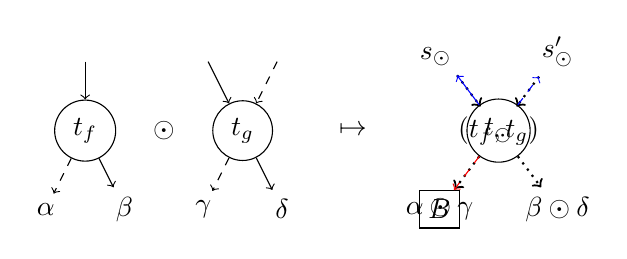
\begin{tikzpicture}
      % 'f'
      \node[shape = circle, draw = black] at (0,0) (f) {$t_f$};

      \node at (-0.5,-1) (f0) {$\alpha$};
      \node at (0.5,-1) (f1) {$\beta$};

      \draw[->, dashed] (f) edge (f0);
      \draw[->]         (f) edge (f1);

      \node at (0,1) (fp) {};
      \draw[->] (fp) edge (f);

      % 'odot'
      \node at (1,0) {$\odot$};

      % 'g'
      \node[shape = circle, draw = black] at (2,0) (g) {$t_g$};

      \node at (1.5,-1) (g0) {$\gamma$};
      \node at (2.5,-1) (g1) {$\delta$};

      \draw[->, dashed] (g) edge (g0);
      \draw[->]         (g) edge (g1);

      \node at (1.5,1) (gp0) {};
      \node at (2.5,1) (gp1) {};
      \draw[->] (gp0) edge (g);
      \draw[->, dashed] (gp1) edge (g);

      \node at (3.4,0) {$\mapsto$};

      % 'f \odot g' (before)
      \node at (4.5,1) (fgp0) {$s_{\odot}\phantom{'}$};
      \node at (6.0,1) (fgp1) {$s_{\odot}'$};

      \onslide<1>{
        \node at (5.25,0) (fg) {$(t_f,t_g)$};

        \draw[->, dotted, thick] (fgp0) edge (fg);
        \draw[->, dotted, thick] (fgp1) edge (fg);
      }

      % 'f \odot g' (after)
      \onslide<2->{
        \node[shape = circle, draw = black] at (5.25,0) (fg) {$t_{\odot}$};

        \draw[blue, ->]         (fg) edge (fgp0);
        \draw[blue, ->, dashed] (fg) edge (fgp1);
      }
      \onslide<3->{
        \node at (6,-1) (fg1) {$\beta \odot \delta$};
        \draw[->, dotted, thick] (fg) edge (fg1);
      }
      \onslide<3>{
        \node at (4.5,-1) (fg0) {$\alpha \odot \gamma$};
        \draw[->, dotted, thick] (fg) edge (fg0);
      }
      \onslide<4>{
        \node[shape=rectangle, draw=black] at (4.5,-1) (fg0) {$\B$};
        \draw[->, red, dashed] (fg) edge (fg0);
      }
    \end{tikzpicture}
  \end{figure}

  \onslide<2->{{\bf Observation (semi-tranposition)}}
  \begin{itemize}
    \onslide<2->{
    \item[{\color{blue} $\leftarrow$} :]{\color{blue} $\arc{s}{}{t}$}\hspace{3pt}
      (Internal Arcs) are output at time $t$ and hence sorted by $t$.
    }

    \onslide<4->{
    \item[{\color{red} $\rightarrow$} :] {\color{red} $\arc{s}{}{\B}$} (Terminal
      Arcs) are output at time $s$.
    }
  \end{itemize}

  \begin{center}
    {\Large \textbf{Time-Forward Processing}}

    Defer resolving products with $Q_{\mathit{app}:1}$, $Q_{\mathit{app}:2}$ :
    \texttt{PriorityQueue}$\langle (\arc{s}{}{(t_f,t_g)}, ...) \rangle$.
  \end{center}
\end{frame}

\begin{frame}[t]
  \frametitle{Apply}

  % priority queues
  \begin{columns}
    \begin{column}{0.46\linewidth}
      $Q_{\mathit{app}:1}$: \texttt{PriorityQueue}$\langle
      (\arc{s}{}{(t_f, t_g)}) \rangle$ sorted on $\min(t_f, t_g)$ in ascending
      order.
    \end{column}
    \begin{column}{0.54\linewidth}
      \onslide<3>{%
        $Q_{\mathit{app}:2}$: \texttt{PriorityQueue}$\langle (\arc{s}{}{(t_f,
          t_g)}, (\alpha, \beta)) \rangle$ sorted on $\max(t_f, t_g)$ in
        ascending order.
      }
    \end{column}
  \end{columns}

  \vspace{10pt}

  % cases
  \begin{columns}[T]
    \begin{column}{0.46\linewidth}
      \textbf{Case 1\phantom{(a)}:}

      $t_f.\mathit{var}() \neq t_g.\mathit{var}()$

      \vspace{10pt}

      \begin{figure}
        \centering

        \begin{tikzpicture}[scale=0.8]
          \node[shape = circle, draw = black] (tf) {$t_f$};

          \node[below left  = 0.5 and 0.2 of tf] (alpha) {$\alpha$};
          \node[below right = 0.5 and 0.2 of tf] (beta)  {$\beta$};

          \node[shape = circle, draw = black, below right=0 and 2.7 of tf] (tg) {$t_g$};

          \node[below left  = 0.5 and 0.2 of tg] (gamma) {$\gamma$};
          \node[below right = 0.5 and 0.2 of tg] (delta) {$\delta$};

          \node[left=2 of tf] (p) {};

          \draw[->, dashed]
            (tf) edge (alpha)
            (tg) edge (gamma)
          ;
          \draw[->]
            (tf) edge (beta)
            (tg) edge (delta)
          ;

          \draw[->, densely dotted, thick]
            (p) edge[bend left] node[above] {$Q_{\mathit{app}:1}$} (tf)
          ;
        \end{tikzpicture}
      \end{figure}
    \end{column}
    \begin{column}{0.54\linewidth}
      \onslide<2->{%
        \textbf{Case 2(a):}

        $t_f.\mathit{var}() = t_g.\mathit{var}() \wedge t_f.\mathit{id}() =
        t_g.\mathit{id}()$
      }

      \vspace{5pt}

      \onslide<3>{%
        \textbf{Case 2(b):}

        $t_f.\mathit{var}() = t_g.\mathit{var}() \wedge t_f.\mathit{id}() \neq
        t_g.\mathit{id}()$

        \begin{figure}
          \centering

          \begin{tikzpicture}[scale=0.8]
            \node[shape = circle, draw = black] (tf) {$t_f$};

            \node[below left  = 0.5 and 0.2 of tf] (alpha) {$\alpha$};
            \node[below right = 0.5 and 0.2 of tf] (beta)  {$\beta$};

            \node[shape = circle, draw = black, right= 2 of tf] (tg) {$t_g$};

            \node[below left  = 0.5 and 0.2 of tg] (gamma) {$\gamma$};
            \node[below right = 0.5 and 0.2 of tg] (delta) {$\delta$};

            \node[left=2 of tf] (p) {};

            \draw[->, dashed]
              (tf) edge (alpha)
              (tg) edge (gamma)
            ;
            \draw[->]
              (tf) edge (beta)
              (tg) edge (delta)
            ;

            \draw[->, densely dotted, thick]
              (p) edge[bend left] node[above] {$Q_{\mathit{app}:1}$} (tf)
              (tf) edge[bend left] node[above] {$Q_{\mathit{app}:2}$} (tg)
            ;
          \end{tikzpicture}
        \end{figure}
      }
    \end{column}
  \end{columns}
\end{frame}

\begin{frame}
  \frametitle{Apply : \emph{Example}}

  % NOTE: The algorithm as presented here has a bug; for more information read
  % the note within the animation file.

  \input{anim/apply_tfp.tex}
\end{frame}

\begin{frame}
  \frametitle{Apply}

  \setvalue{tandem_apply  = lightgray}
  \setvalue{tandem_reduce = black}

  \input{tikz/tandem.tex}
\end{frame}

\begin{frame}
  \frametitle{Apply (Reduce)}

  \begin{figure}
    \centering

    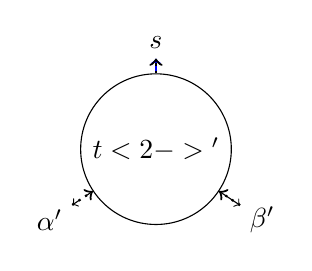
\begin{tikzpicture}[scale=0.9]
      \node[shape = circle, draw = black] at (0,0) (t) {$t\onslide<2->{'}$};

      \node at (-1.5,-1) (t0) {$\alpha'$};
      \node at ( 1.5,-1) (t1) {$\beta'$};

      \node at ( 0, 1.5) (s) {$s$};

      \onslide<1>{
        \draw[->, dotted, thick]
          (t0) edge (t)
          (t1) edge (t)
        ;
      }
      \onslide<1-2>{
        \draw[blue, ->] (t) edge (s);
      }
      \onslide<2->{
        \draw[->, dashed] (t) edge (t0);
        \draw[->]         (t) edge (t1);
      }
      \onslide<3->{
        \draw[->, dotted, thick] (t) edge (s);
      }
    \end{tikzpicture}
  \end{figure}

  \begin{center}
    {\Large \textbf{Time-Forward Processing}}

    Send reduction $t'$ with $Q_{\mathit{red}}$ : \texttt{PriorityQueue}$\langle
    (\arc{s}{}{t'}) \rangle$ descending on parent $s$.
  \end{center}

  \onslide<3->{{\bf Observation (semi-tranposition)}}
  \begin{itemize}
    \onslide<3->{
    \item[{\color{blue} $\leftarrow$} :]{\color{blue} $\arc{s}{}{t}$}\hspace{3pt}
      (Internal Arcs) provide parents of unreduced node $t$.
    }

    \onslide<4->{
    \item[{\color{red} $\rightarrow$} :] {\color{red} $\arc{s}{}{\B}$} (Terminal
      Arcs) are reduced and already sorted as per $Q_{\mathit{red}}$.
    }
  \end{itemize}
\end{frame}

\begin{frame}
  \frametitle{Apply (Reduce)}

  \input{anim/reduce_level.tex}

  \textbf{Reduce Level $i$}:
  \begin{enumerate}
    \onslide<1->{%
    \item Obtain nodes from $Q_{\mathit{red}}$ and {\color{red} terminal
        arcs}. Filter and {\color{purple} remember} redundant nodes.
    }%
    \onslide<4->{%
    \item Sort remaining nodes by children, output unique nodes, and
      {\color{purple} remember} duplications.
    }%
    \onslide<6->{%
    \item Sort back to match {\color{blue} internal arcs} and forward to parents
      with $Q_{\mathit{red}}$.
    }%
  \end{enumerate}
\end{frame}

\begin{frame}
  \frametitle{Apply (Reduce) : \emph{Example}}

  \input{anim/reduce_tfp.tex}
\end{frame}

\begin{frame}
  \begin{table}
    \centering
    \begin{tabular}{rl}
      Algorithm                 & I/O-Complexity
      \\ \hline \hline
      \lstinline{bdd_pathcount} & $O(\sort(N_f))$
      \\ \hline
      \lstinline{bdd_not}       & $2 N_f / B$
      \\
      \lstinline{bdd_restrict}  & $O(\sort(N_f))$
      \\
      \lstinline{bdd_apply}     & $O(\sort(N_f \cdot N_g))$
    \end{tabular}
  \end{table}
\end{frame}

\begin{frame}
  \begin{figure}
    \centering

    \begin{tikzpicture}
      \begin{axis}[%
        width=0.70\linewidth, height=0.42\linewidth,
        every tick label/.append style={font=\scriptsize},
        % x-axis
        xlabel={number of BDD nodes},
        xmajorgrids=true,
        xmin=51000000,
        xmax=300000000000,
        xmode = log,
        % y-axis
        ymin=0,
        ymax=2.2,
        ytick distance={0.5},
        ylabel={$\mu$s / BDD node},
        yminorgrids=true,
        ymajorgrids=true,
        grid style={dashed,black!20},
        ]

        \only<1-> {
          \addplot+ [style=plot_buddy]
          table {./data/queens_buddy_time_per_node.tex};
        }
        \only<1-> {
          \addplot+ [style=plot_cudd]
          table {./data/queens_cudd_time_per_node.tex};
        }
        \only<1-> {
          \addplot+ [style=plot_sylvan]
          table {./data/queens_sylvan_time_per_node.tex};
        }

        \only<2-> {
          \addplot+ [style=plot_adiar]
          table {./data/queens_adiar_time_per_node.tex};
        }
      \end{axis}

    \end{tikzpicture}

    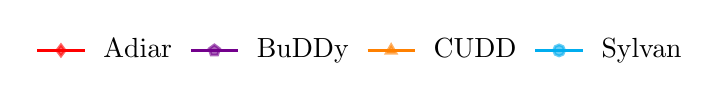
\begin{tikzpicture}
      \begin{customlegend}[
        legend columns=-1,
        legend style={draw=none,column sep=1ex},
        legend entries={Adiar, BuDDy, CUDD, Sylvan}
        ]
        \addlegendimage{style=plot_adiar}
        \addlegendimage{style=plot_buddy}
        \addlegendimage{style=plot_cudd}
        \addlegendimage{style=plot_sylvan}
      \end{customlegend}
    \end{tikzpicture}

    \caption{Running time for the $N$-\emph{Queens} problems.}
  \end{figure}
\end{frame}

\subsection{Equality Checking}

\begin{frame}[plain,noframenumbering]{}
  \frametitle{Contents}
  \tableofcontents[currentsection, currentsubsection]
\end{frame}

\begin{frame}
  \begin{table}
    \centering
    \begin{tabular}{rl}
      Algorithm                 & I/O-Complexity
      \\ \hline \hline
      \lstinline{bdd_pathcount} & $O(\sort(N_f))$
      \\ \hline
      \lstinline{bdd_not}       & $2 N_f / B$
      \\
      \lstinline{bdd_restrict}  & $O(\sort(N_f))$
      \\
      \lstinline{bdd_apply}     & $O(\sort(N_f \cdot N_g))$
                                  \pause
      \\ \hline
      \lstinline{bdd_equal}     & ?
    \end{tabular}
  \end{table}
\end{frame}

\begin{frame}
  \frametitle{Equality Checking}

  \vspace{30pt}
  \begin{center}
    {\huge $f \leftrightarrow g \equiv \top$}
  \end{center}

  \pause
  \vspace{20pt}

  \begin{equation*}
    \underbrace{O(\sort(N^2))}_{\texttt{Apply}}
    + \underbrace{O(\sort(N^2))}_{\texttt{Reduce}}
    + \underbrace{O(1))}_{\text{check is } \top}
    = O(\sort(N^2))
  \end{equation*}
\end{frame}

\begin{frame}[t]
  \frametitle{Equality Checking}

  \begin{theorem}[Bryant '86]
    Let $\pi$ be a variable order and $f : \B^n \rightarrow \B$ then there
    exists a unique (up to isomorphism) Reduced Ordered Binary Decision
    Diagram representing $f$ with ordering $\pi$.
  \end{theorem}

  \pause
  {\bf Trivial cases: $f \not \equiv g$ if there is a mismatch in}

  \begin{tabular}{c l l l}
    {\tiny $\blacksquare$} & $N_f \neq N_g$       & Number of nodes            & $O(1)$ I/Os
    \\
    {\tiny $\blacksquare$} & $L_f \neq L_g$       & Number of levels           & $O(1)$ I/Os
    \\
    {\tiny $\blacksquare$} & $N_{f,i} \neq N_{g,i}$ & Number of nodes on a level & $O(L/B)$ I/Os
    \\
    {\tiny $\blacksquare$} & $L_{f,i} \neq L_{g,i}$ & Label of an $i$th level    & $O(L/B)$ I/Os
  \end{tabular}
\end{frame}

\begin{frame}[t]
  \frametitle{Equality Checking}

  % TODO: code duplication
  \begin{theorem}[Bryant '86]
    Let $\pi$ be a variable order and $f : \B^n \rightarrow \B$ then there
    exists a unique (up to isomorphism) Reduced Ordered Binary Decision
    Diagram representing $f$ with ordering $\pi$.
  \end{theorem}

  \begin{figure}
    \centering

    \begin{tikzpicture}[scale=1, every node/.style={transform shape}]
      \input{anim/isomorphism_local_violation.tex}
    \end{tikzpicture}
  \end{figure}

\end{frame}

\begin{frame}[t]
  \frametitle{Equality Checking}

  % TODO: code duplication
  \begin{theorem}[Bryant '86]
    Let $\pi$ be a variable order and $f : \B^n \rightarrow \B$ then there
    exists a unique (up to isomorphism) Reduced Ordered Binary Decision
    Diagram representing $f$ with ordering $\pi$.
  \end{theorem}

  \texttt{IsIsomorphic($f$, $g$)}
  \begin{itemize}
  \item Check whether root $v_f$ of $f$ and root $v_g$ of $g$ have a local violation.
  \item Check $\mathit{low}(v_f) \sim \mathit{low}(v_g)$ and $\mathit{high}(v_f)
    \sim \mathit{high}(v_g)$ ``recursively''.
  \end{itemize}
  Return \texttt{false} on first violation. If there are no violations then return \texttt{true}.
  \pause
  \begin{equation*}
    \underbrace{O(\sort(N^2))}_{\texttt{Apply}'}
    + \underbrace{\hcancel[gray]{O(\sort(N^2))}}_{\texttt{Reduce}}
    + \underbrace{\hcancel[gray]{O(1))}}_{\text{check is } \top}
    =
    O(\sort(N^2))
  \end{equation*}
\end{frame}

\begin{frame}[t]
  \frametitle{Equality Checking}

  % TODO: code duplication
  \begin{theorem}[Bryant '86]
    Let $\pi$ be a variable order and $f : \B^n \rightarrow \B$ then there
    exists a unique (up to isomorphism) Reduced Ordered Binary Decision
    Diagram representing $f$ with ordering $\pi$.
  \end{theorem}

  \vspace{-10pt}
  \begin{figure}
    \centering

    \begin{tikzpicture}[scale=0.9, every node/.style={transform shape}]
      \input{tikz/isomorphism_level_fail.tex}
    \end{tikzpicture}
  \end{figure}
  \pause
  \vspace{-20pt}
  Return \texttt{false} if more than $N_{f,i} = N_{g,i}$ pairs of nodes are checked on level $i$.
  \begin{equation*}
    \underbrace{O (\sort (\Sigma_{i}\ N_{f,i} ) )}_{\texttt{Apply}''}
    =
    O(\sort(N))
  \end{equation*}
\end{frame}

\begin{frame}
  \frametitle{Equality Checking}

  \input{anim/reduce_prop.tex}

  {\bf Observation}

  \vspace{-10pt}
  Each level output by the \texttt{Reduce} algorithm has the following properties:
  \begin{itemize}
    \onslide<4->{
    \item Nodes on level $i$ have their identifiers \emph{consecutively} numbered.
    }
    \onslide<6->{
    \item Nodes on level $i$ are output sorted by their children.
    }
  \end{itemize}
\end{frame}

\begin{frame}
  \frametitle{Equality Checking}

  \begin{theorem}
    If $G_f$ and $G_g$ are outputs of \lstinline{Reduce}.
    \begin{center}
      $G_f \sim G_g$ $\iff$ For all $i \in [0; N_f)$ the node $G_f[i]$ matches
      $G_g[i]$ numerically.
    \end{center}
  \end{theorem}
  \begin{proof}
    $\Leftarrow$ : Must describe the exact same graph.

    $\Rightarrow$ : Strong induction on BDD levels bottom-up.
  \end{proof}

  \pause
  \begin{corollary}
    If $G_f$ and $G_g$ are outputs of \lstinline{Reduce} then $f \equiv g$ is
    computable using $2 \cdot N/B$ I/Os.
  \end{corollary}
\end{frame}


\begin{frame}
  \frametitle{Equality Checking}

  \begin{table}
    \centering
    \begin{tabular}{r | l}
      Algorithm                         & Time (s)
      \\ \hline
      $f \leftrightarrow g \equiv \top$ & 0.38
      \\ \onslide<2->{
      $O(\sort(N))$                     & 0.058}
      \\ \onslide<3->{
      $2N/B$                            & 0.006}
    \end{tabular}

    \caption{Checking the (EPFL Benchmark) \emph{voter} circuit's single output
      gate ($\abs{N_f} = \abs{N_g} = 5.76~\text{MiB}$).}
  \end{table}
\end{frame}

\blankframe

\begin{frame}[plain,noframenumbering]
  % custom copy of fram/endslate.tex
  \begin{columns}
    \begin{column}{0.42\linewidth}
      {\Large \textbf{Steffan Christ S{\o}lvsten}}
      \vspace{1pt} {\hrule width\linewidth}

      \vspace{5pt}

      \begin{itemize}
      \item[\faIcon{envelope}] \mailto{soelvsten@cs.au.dk}
      \item[\faIcon{globe}] \href{https://ssoelvsten.github.io}{ssoelvsten.github.io}
      \end{itemize}

      \vspace{10pt}

      {\Large \textbf{Adiar}}
      \vspace{1pt} {\hrule width\linewidth}

      \vspace{5pt}

      \begin{itemize}
      \item[\faIcon{code}]
        \href{http://github.com/ssoelvsten/adiar}{github.com/ssoelvsten/adiar}
      \item[\faIcon{book}\hspace{2pt}]
        \href{http://ssoelvsten.github.io/adiar}{ssoelvsten.github.io/adiar}
      \end{itemize}

      \vspace{10pt}

      \includegraphics[width=0.5\linewidth]{external/aulogo_uk_var2_black.eps}
    \end{column}
    \begin{column}{0.57\linewidth}
      \centering
      \begin{tabular}{rll}
        Algorithm                 & Depth-First  & Time-Forwarding
        \\ \hline \hline
        \lstinline{bdd_pathcount} & $O(N_f)$     & $O(\sort(N_f))$
        \\ \hline
        \lstinline{bdd_not}       & $O(N_f)$     & $2 N_f / B$
        \\
        \lstinline{bdd_restrict}  & $O(N_f)$     & $O(\sort(N_f))$
        \\
        \lstinline{bdd_apply}     & $O(N_f N_g)$ & $O(\sort(N_f  N_g))$
        \\ \hline
        \lstinline{bdd_equal}     & $O(1)$       & $2 N/B$
      \end{tabular}

      \vspace{60pt}
    \end{column}
  \end{columns}

\end{frame}

\end{document}

%%% Local Variables:
%%% mode: latex
%%% TeX-master: t
%%% End:
